The next figures show the result of submit a beam to a load and break static test;
thus, a system setup like the one described in the Sec. \ref{sec:systemdesc} was used.
The test results were captures using two methods,
the first method uses dial watches and the second apply the $PIV$ technique (see Sec. \ref{sec:algorithm}) over 
$M=19$ pictures, as described in the Sec. \ref{subsec:syssetup} following the procedure described
in the Algorithm \ref{alg:PIV}, with the consideration that in the pictures, $1$ pixel is
equivalent to $0.27027$ millimeters.

In the test, the  dial indicators will return the maximum deformation of the beam,
as it is shown in the Table \ref{tab:watch}. The Figs. \ref{fig:pivwindow} and  \ref{fig:system1}
describe the disposition of these indicators, where  the \textit{dial indicator 0}, \textit{dial indicator 1} 
and \textit{dial indicator 2} represent the indicators in the left, middle and the right, respectively.

\begin{table}[h]
  \begin{tabular}{ p{0.18\columnwidth} | p{0.18\columnwidth} | p{0.18\columnwidth} | p{0.18\columnwidth}}
    \hline
    ~                  & Dial indicator 0 & Dial indicator 1 & Dial indicator 2 \\ \hline \hline
   Maximum deformation & 6.75 mm & 11.29 mm & 6.9 mm \\ \hline
    
  \end{tabular}
  \caption{Beam deformation measure with the dial indicators. }
  \label{tab:watch}
\end{table}

On the other hand, using the $PIV$ technique, we select the analysis regions as showed in the
left image of Fig. \ref{fig:pivwindow}.   Dislocation
and rotation tests were apply over these analysis regions, 
as described in the Algs. \ref{alg:displacementtest} and \ref{alg:rotationtest},
respectively. The results of displacement tests can be seen in the 
Figs. \ref{fig:numresult1-des} and  \ref{fig:numresult1-des-max}.
It is easy to see in the Fig. \ref{fig:numresult1-des-max} 
that if there was only a displacement process over the analysis regions,
then it will be necessary to have a $l_0\sqrt{2}/2<2$ pixels ($l_0<2.8284$) 
to not exist a possibility of a false positive, in 
the recognition process, with a region located around of $17$ or $18$ pixels of neighborhood.
\begin{figure}[H]
\centering
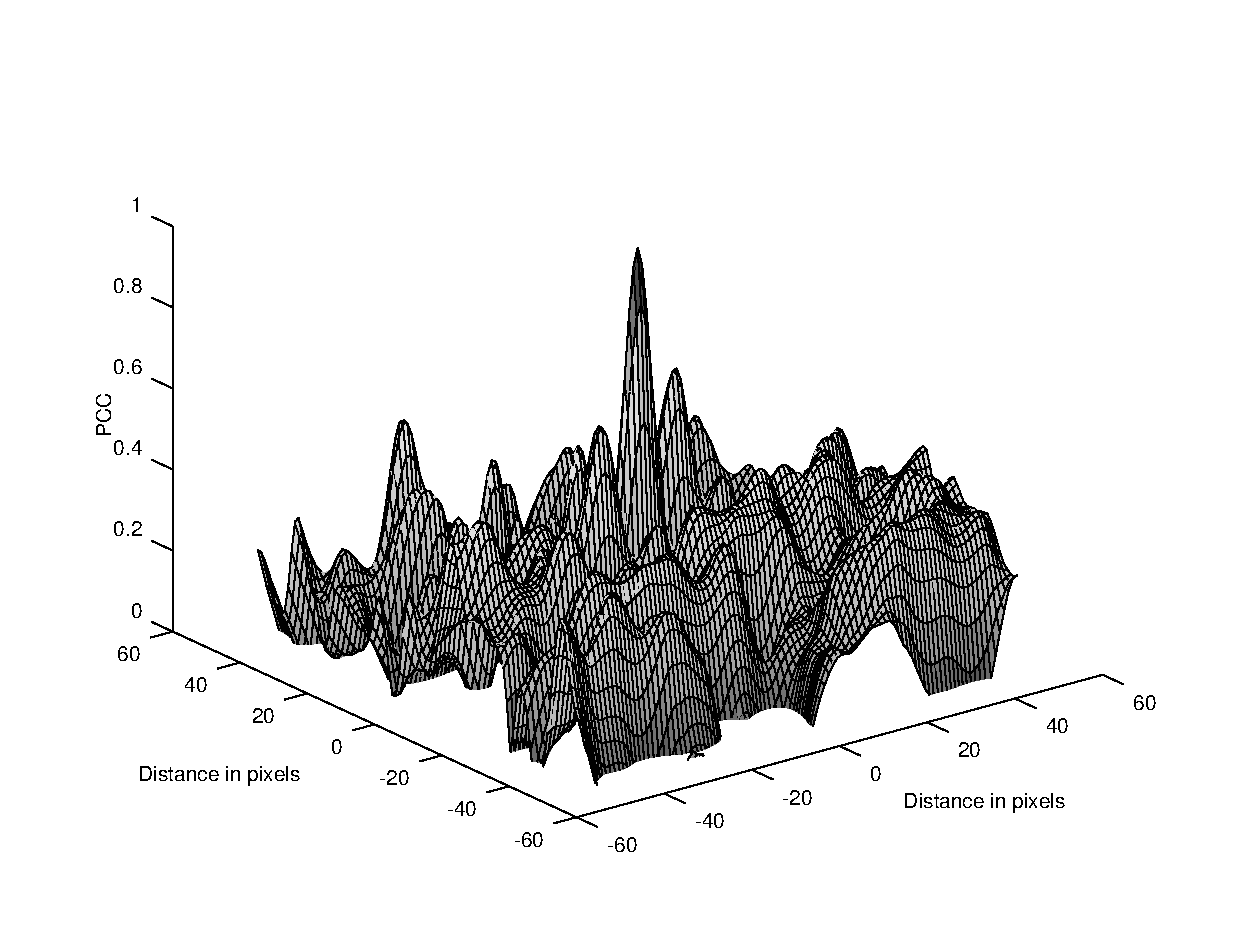
\includegraphics[width=\columnwidth]{PCC-Point0-multi_des.eps}
\caption{Displacement tests over the analysis region 0.}
\label{fig:numresult1-des}
\end{figure}
\begin{figure}[H]
\centering
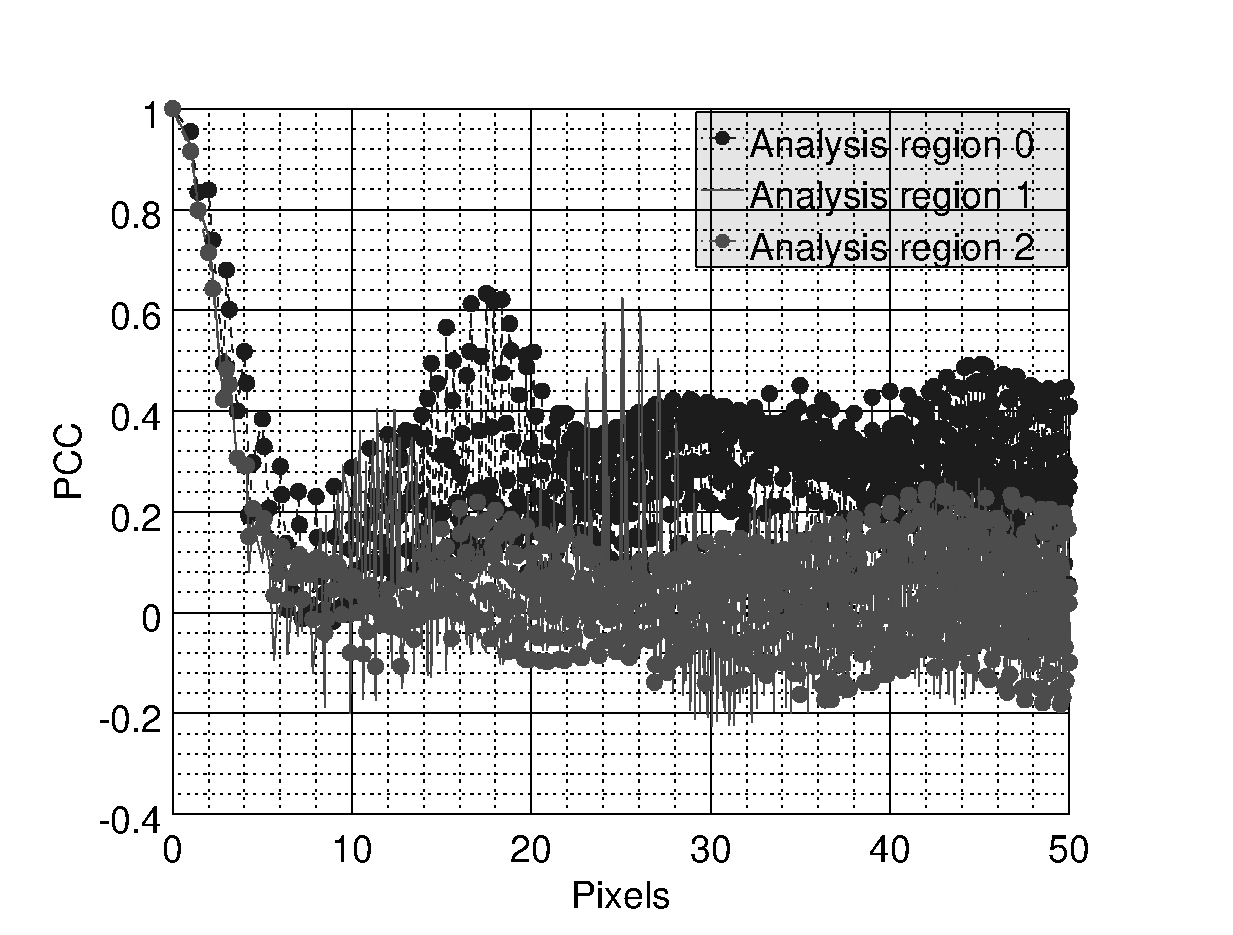
\includegraphics[width=\columnwidth]{numresult1-maketestjoint-multi_des_max.eps}
\caption{Displacement tests over the selected analysis regions showed in the radius form.}
\label{fig:numresult1-des-max}
\end{figure}

Additionally, the results of rotation test can be seen in the Fig. \ref{fig:numresult1-rot};
in this graphic it is easy to see that if there is only a rotation process over the 
analysis regions then on average the $PCC$ value decrease with the angle ($\alpha$ in degrees) 
following approximately the function $e^{-\left( \alpha/14\right)^2}$. Knowing that
the beam in last image has a horizontal rotation of $4.5^\circ$, then we can calculate that 
the mean rotation angle between the analysis region, of two consecutive images, 
is $0.25^\circ$, equivalent to a decrease of $PCC$ at $0.99972$.
\begin{figure}[H]
\centering
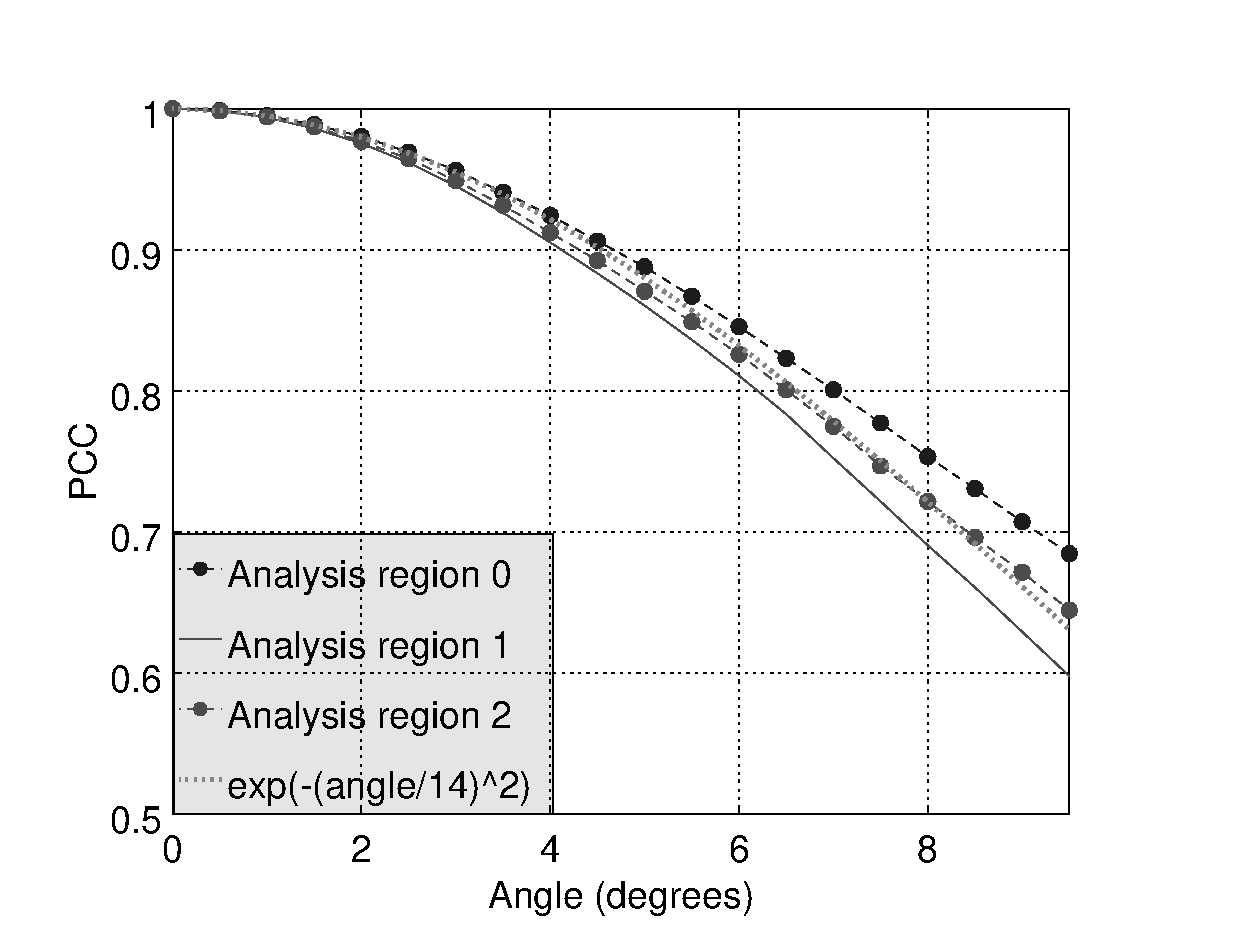
\includegraphics[width=\columnwidth]{numresult1-maketestjoint-rot.eps}
\caption{Rotation tests over the selected analysis regions.}
\label{fig:numresult1-rot}
\end{figure}
Thus, in the cases of analysis regions and pictures used, 
the procedure made between two images that most influence 
in the loss of correlation is the dislocation.


Using these results we can estimate that if we use the parameters:
$T=0.6$, $l_0=4$, $L=50$ and $WSIZE=32$, we are open to the possibility of introducing
error in the $PIV$ technique.
So that, for a $l_0=4$ the bi-dimensional measure error between images is at most $2.8284$ pixels 
(equivalent to $0.76444$ millimeters). Following the results in the 
Fig. \ref{fig:numresult1-des-max} for a measure error of $2.8284$ the $3$
analysis regions are located 
slightly above (analysis region 0), and 
slightly bellow (analysis regions 1 and 2) of the threshold $T=0.6$.
Thus, the analysis regions 1 and 2 are automatically discarded because they are below the threshold, 
furthermore the analysis region 0 is above the  threshold but has a $PCC$
value so close to a $PCC$ of a false positive located around of $17$ or $18$ pixels of neighborhood.
These considerations highlight that there will be errors in the results of $PIV$ 
algorithm, as it can be seen in the Fig. \ref{fig:numresult1testb} when compared to Table \ref{tab:watch}.

\begin{figure}[H]
\centering
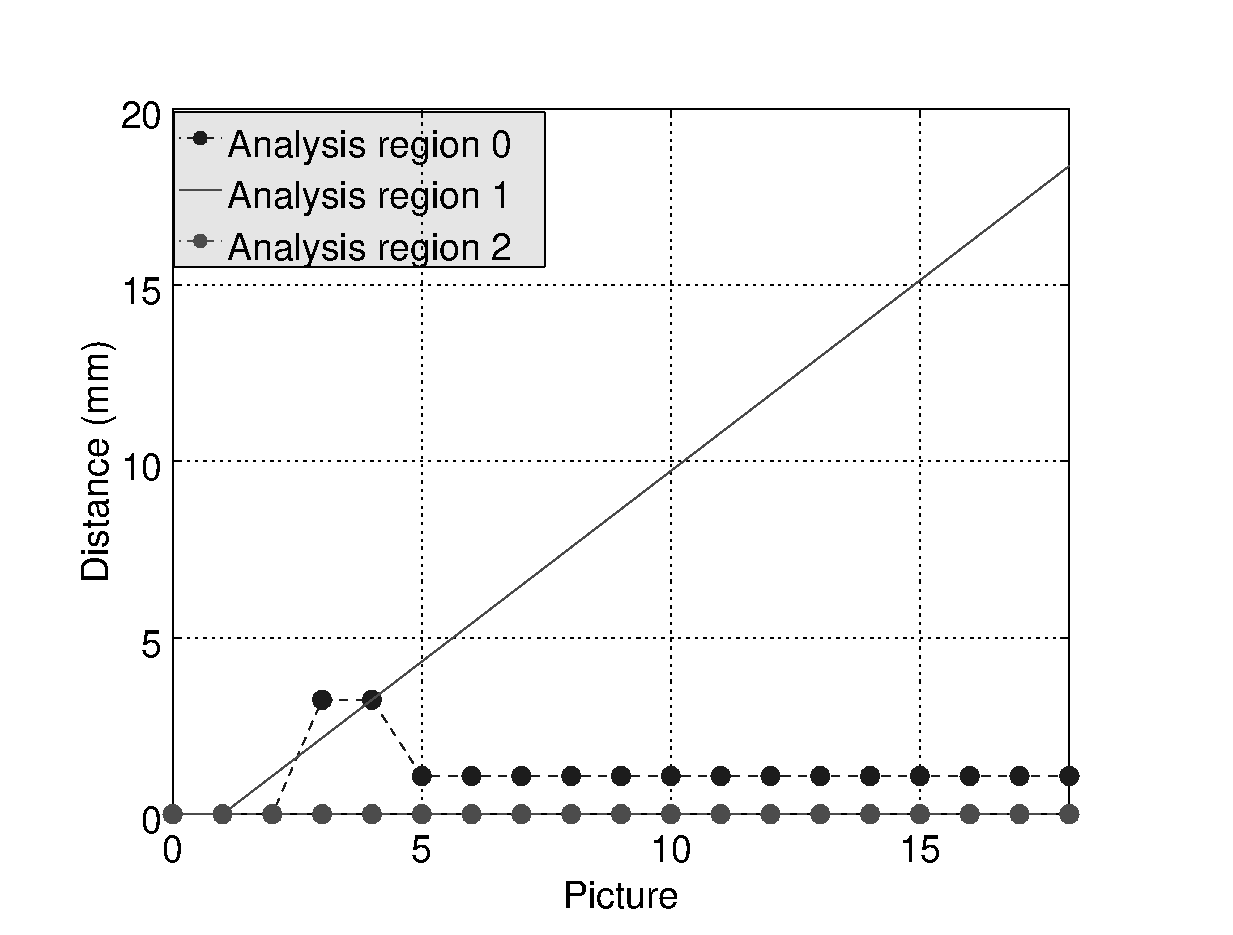
\includegraphics[width=\columnwidth]{numresult1-test-b.eps}
\caption{Tracking results of $PIV$ method over the selected analysis regions, with $l_0=4$ and $T=0.60$.}
\label{fig:numresult1testb}
\end{figure}


Moreover, we can estimate that if we use the parameters,
$T=0.82$, $l_0=1$, $L=50$ and $WSIZE=32$, we to get better results,
given that to a $l_0=1$ the bi-dimensional measure error is at most $0.70711$ pixels 
(equivalent to $0.19111$ millimeters).
Following the results in the Fig. \ref{fig:numresult1-des-max} 
to a measure error of $0.70711$ we can see that the $PCC$ value of the $3$
analysis regions are located much above of threshold $T=0.82$ and additionally
there is not the possibility of a false positive with any other group of pixels
because the unique pixels group that is above the threshold is the pixels group in a radius
of $0.70711$ pixels of origin.
Thus, with a measure error of $e=0.70711$ pixels across of $M=19$ images,
the maximum possible measure error in the $PIV$ technique will be $(M-1)e \equiv 12.728$ pixels
(in this case equivalent to $3.4400$ millimeters).
In the Fig. \ref{fig:numresult1testa} we can see th results of $PIV$ technique using these parameters,
if we compare these results to Table \ref{tab:watch} it is easy to see that the values are to close.
Table \ref{tab:watch2} presents this in detail, where are the maximum error is $0.60200 < 3.4400$ millimeters.
\begin{figure}[H]
\centering
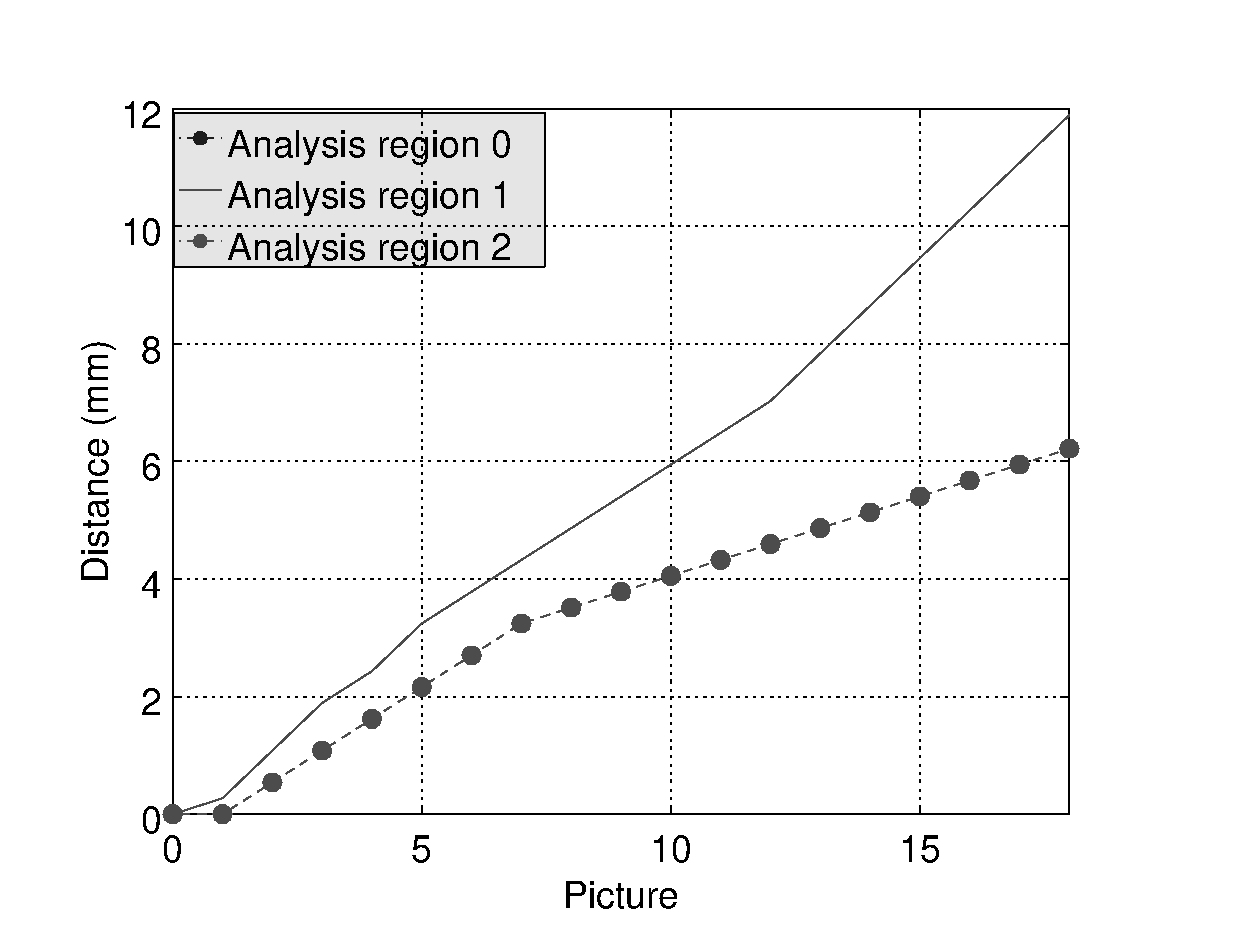
\includegraphics[width=\columnwidth]{numresult1-test-a.eps}
\caption{Tracking results of $PIV$ method over the selected analysis regions, with $l_0=1$ and $T=0.82$.}
\label{fig:numresult1testa}
\end{figure}

\begin{table}[h]
  \begin{tabular}{ p{0.18\columnwidth} | p{0.18\columnwidth} | p{0.18\columnwidth} | p{0.18\columnwidth}}
    \hline
    Error in      & Dial indicator 0 & Dial indicator 1 & Dial indicator 2 \\ \hline \hline
%    value & 6.2162 mm & 11.892 mm & 6.2162 mm \\ \hline
    millimeters & 0.5338 mm & 0.6020 mm & 0.6838 mm \\ \hline
    percentage  & 7.9081 \% & 5.3322 \% & 9.9101 \% \\ \hline
    
  \end{tabular}
  \caption{Error in the measure of beam deformation with the $PIV$ technique when compared with the dial indicators.}
  \label{tab:watch2}
\end{table}

